\documentclass[12pt,a4paper]{article}

% ─── Page Layout ───────────────────────────────────────────────────────────────
\usepackage[a4paper, margin=0.8in, headheight=14pt]{geometry}

% ─── Fonts (XeLaTeX) ───────────────────────────────────────────────────────────
\usepackage{fontspec}
\usepackage{unicode-math}
\setmainfont{TeX Gyre Pagella}
\setmonofont[Scale=0.88]{TeX Gyre Cursor}
\setmathfont{Latin Modern Math}

% ─── Packages ──────────────────────────────────────────────────────────────────
\usepackage{xcolor}
\usepackage{colortbl}
\usepackage{titlesec}
\usepackage{enumitem}
\usepackage{tabularx}
\usepackage{booktabs}
\usepackage{array}
\usepackage{amsmath}
\usepackage{tikz}
\usetikzlibrary{shapes.geometric, arrows.meta, positioning, calc, fit, decorations.pathreplacing}
\usepackage{tcolorbox}
\tcbuselibrary{skins, breakable}
\usepackage{hyperref}
\usepackage{fancyhdr}
\usepackage{graphicx}
\usepackage{microtype}
\hyphenpenalty=10000
\exhyphenpenalty=10000
\sloppy
\usepackage{caption}
\usepackage{setspace}
\usepackage{multirow}
\usepackage{tocloft}

% ─── Q&A helper ────────────────────────────────────────────────────────────────
\newcommand{\Q}[1]{\textbf{#1}\par\noindent\ignorespaces}

% ─── Colour Palette ────────────────────────────────────────────────────────────
\definecolor{myred}{RGB}{196,30,58}
\definecolor{mydark}{RGB}{30,30,50}
\definecolor{mygreen}{RGB}{14,120,80}
\definecolor{myteal}{RGB}{0,130,140}
\definecolor{myamber}{RGB}{180,100,0}
\definecolor{mypurple}{RGB}{100,30,160}
\definecolor{mygray}{RGB}{246,247,249}
\definecolor{mgframe}{RGB}{180,185,200}
\definecolor{watermark}{RGB}{145,150,170}
\definecolor{hdrred}{RGB}{250,232,235}
\definecolor{hdrgreen}{RGB}{220,244,233}
\definecolor{hdrteal}{RGB}{220,242,244}
\definecolor{hdramber}{RGB}{253,242,215}
\definecolor{hdrpurple}{RGB}{238,228,255}
\definecolor{hdrgray}{RGB}{238,240,245}
\definecolor{rowalt}{RGB}{250,251,253}

% ─── Section Formatting ────────────────────────────────────────────────────────
\titleformat{\section}
  {\large\bfseries\color{myred}}{\thesection.}{0.5em}{}
  [\vspace{1pt}{\color{myred}\rule{\linewidth}{0.8pt}}]
\titleformat{\subsection}
  {\normalsize\bfseries\color{myteal}}{\thesubsection}{0.5em}{}
\titlespacing*{\section}{0pt}{18pt}{7pt}
\titlespacing*{\subsection}{0pt}{11pt}{4pt}

% ─── Paragraph ─────────────────────────────────────────────────────────────────
\setlength{\parindent}{0pt}
\setlength{\parskip}{4pt}

% ─── TOC Styling ───────────────────────────────────────────────────────────────
\renewcommand{\cfttoctitlefont}{\large\bfseries\color{myred}}
\renewcommand{\cftaftertoctitle}{\par\noindent{\color{myred}\rule{\linewidth}{0.8pt}}}
\setlength{\cftbeforetoctitleskip}{0pt}
\setlength{\cftaftertoctitleskip}{6pt}
\renewcommand{\cftsecfont}{\normalsize\bfseries\color{mydark}}
\renewcommand{\cftsecpagefont}{\normalsize\bfseries\color{mydark}}
\renewcommand{\cftsecleader}{\cftdotfill{\cftdotsep}}
\setlength{\cftbeforesecskip}{7pt}
\renewcommand{\cftsubsecfont}{\small\color{mydark}}
\renewcommand{\cftsubsecpagefont}{\small\color{mydark}}
\setlength{\cftbeforesubsecskip}{3pt}
\setlength{\cftsubsecindent}{1.4em}

% ─── Table helpers ─────────────────────────────────────────────────────────────
\renewcommand{\arraystretch}{1.45}
\setlength{\tabcolsep}{6pt}
\arrayrulecolor{mydark}
\newcolumntype{B}[1]{>{\small\bfseries\raggedright\arraybackslash}m{#1}}
\newcolumntype{Y}{>{\small\raggedright\arraybackslash}X}
\renewcommand{\tabularxcolumn}[1]{m{#1}}

% ─── Header / Footer ───────────────────────────────────────────────────────────
\pagestyle{fancy}
\fancyhf{}
\fancyhead[L]{\small\color{myred}\textbf{PE-EC702A}\;\color{mydark}--- Adaptive Signal Processing}
\fancyhead[R]{\small\color{myteal}\textbf{Module 1 Notes}}
\fancyfoot[C]{\small\color{mydark}\thepage}
\fancyfoot[R]{\small\color{watermark}\textit{\copyright\ Biraj}}
\renewcommand{\headrulewidth}{0.5pt}
\renewcommand{\footrulewidth}{0.3pt}

% ─── Hyperref ──────────────────────────────────────────────────────────────────
\hypersetup{
  colorlinks=true, linkcolor=myteal, urlcolor=myteal,
  pdfauthor={Biraj Sarkar},
  pdftitle={PE-EC702A --- Module 1 Notes}
}

% ─── tcolorbox styles ──────────────────────────────────────────────────────────
\tcbset{
  tikzbox/.style={
    colback=mygray, colframe=mgframe, boxrule=0.6pt, arc=4pt,
    left=8pt, right=8pt, top=6pt, bottom=6pt,
    colbacktitle=mgframe, coltitle=mydark,
    fonttitle=\small\bfseries
  },
  defbox/.style={
    colback=hdrgreen, colframe=mygreen, boxrule=0.8pt, arc=4pt,
    left=9pt, right=9pt, top=6pt, bottom=6pt,
    colbacktitle=mygreen, coltitle=white,
    fonttitle=\small\bfseries
  },
  formulabox/.style={
    colback=hdrteal, colframe=myteal, boxrule=0.8pt, arc=4pt,
    left=9pt, right=9pt, top=7pt, bottom=7pt,
    colbacktitle=myteal, coltitle=white,
    fonttitle=\small\bfseries
  },
  examplebox/.style={
    colback=hdramber, colframe=myamber, boxrule=0.8pt, arc=4pt,
    left=9pt, right=9pt, top=6pt, bottom=6pt,
    colbacktitle=myamber, coltitle=white,
    fonttitle=\small\bfseries
  },
  masonbox/.style={
    colback=hdrpurple, colframe=mypurple, boxrule=0.8pt, arc=4pt,
    left=9pt, right=9pt, top=6pt, bottom=6pt,
    colbacktitle=mypurple, coltitle=white,
    fonttitle=\small\bfseries
  },
  exambox/.style={
    colback=hdrpurple, colframe=mypurple, boxrule=1pt, arc=5pt,
    left=10pt, right=10pt, top=8pt, bottom=8pt,
    colbacktitle=mypurple, coltitle=white,
    fonttitle=\bfseries,
    breakable, title after break={\textbf{Frequently Asked / Viva Questions (contd.)}}}
}
\tcbset{breakable}

% ─── TikZ styles ───────────────────────────────────────────────────────────────
\tikzset{
  block/.style={rectangle, draw=myteal, fill=hdrteal,
    text width=2.4cm, align=center, minimum height=0.95cm,
    font=\small, rounded corners=3pt, line width=0.7pt},
  redblock/.style={rectangle, draw=myred, fill=hdrred,
    text width=2.4cm, align=center, minimum height=0.95cm,
    font=\small, rounded corners=3pt, line width=0.7pt},
  netnode/.style={rectangle, draw=myteal, fill=hdrteal,
    text width=1.5cm, align=center, minimum height=0.8cm,
    font=\small, rounded corners=3pt, line width=0.7pt},
  sumjunc/.style={circle, draw=myamber, fill=hdramber,
    minimum size=0.62cm, font=\small, line width=0.8pt},
  snode/.style={circle, draw=mypurple, fill=hdrpurple,
    minimum size=0.55cm, font=\footnotesize, line width=0.7pt},
  arrow/.style={-Stealth, thick, color=mydark},
  redarrow/.style={-Stealth, thick, color=myred},
  line/.style={thick, color=mydark}
}

% ═══════════════════════════════════════════════════════════════════════════════
\begin{document}
% ═══════════════════════════════════════════════════════════════════════════════

\begin{center}
  {\LARGE\bfseries\color{myred} PE-EC702A --- Adaptive Signal Processing}\\[5pt]
  {\normalsize\color{mydark} Semester VII \quad$\bullet$\quad 3L:0T:0P \quad$\bullet$\quad 3 Credits}\\[3pt]
  {\normalsize\color{myteal}\textbf{Module 1 Exam Notes: Adaptive Filtering Concepts \& Random Processes}}\\[3pt]
  {\small\color{mydark} CGEC \;$|$\; B.Tech ECE (2023--27) \;$|$\; \textit{Biraj Sarkar}}
\end{center}
\vspace{2pt}
\noindent{\color{myred}\rule{\linewidth}{1.5pt}}
\vspace{2pt}

\hypersetup{linkcolor=mydark}
\tableofcontents
\hypersetup{linkcolor=myteal}
\newpage

% ===============================================================================
\section{General Concept of Adaptive Filtering and Estimation}
% ===============================================================================

An adaptive filter is a self-designing, time-varying system that uses a recursive algorithm to adjust its parameters (coefficients) in order to minimize a predetermined cost function. Unlike fixed linear filters (e.g., standard FIR or IIR filters designed with static cutoff frequencies), adaptive filters automatically adjust to changes in the environment or statistics of the input signals.

\begin{tcolorbox}[defbox]
\textbf{Adaptive Filter:} A digital filter whose transfer function is automatically updated by an adaptive algorithm in response to an incoming error signal, which is computed as the difference between a desired response and the filter's actual output.
\end{tcolorbox}

\subsection{Basic Principles of Operation}
The operations of a typical adaptive filter are structured into two distinct stages:
\begin{enumerate}[label=\textbf{\arabic*.}, leftmargin=*, itemsep=3pt]
  \item \textbf{Filtering Process:} The filter processes an input signal $x(n)$ to produce an output signal $y(n)$. For an $M$-tap transversal (FIR) filter, this is represented by:
  \begin{equation}
    y(n) = \sum_{k=0}^{M-1} w_k(n) x(n-k) = \mathbf{w}^T(n) \mathbf{x}(n)
  \end{equation}
  where $\mathbf{w}(n) = [w_0(n), w_1(n), \dots, w_{M-1}(n)]^T$ is the weight vector, and $\mathbf{x}(n) = [x(n), x(n-1), \dots, x(n-M+1)]^T$ is the input vector.
  \item \textbf{Adaptive Process (Feedback):} An error signal $e(n)$ is generated by comparing the filter output $y(n)$ with a desired response $d(n)$:
  \begin{equation}
    e(n) = d(n) - y(n)
  \end{equation}
  The adaptive algorithm (e.g., LMS or RLS) uses this error $e(n)$ to update the filter coefficients for the next time index:
  \begin{equation}
    \mathbf{w}(n+1) = \mathbf{w}(n) + \Delta \mathbf{w}(n)
  \end{equation}
\end{enumerate}

\subsection{Adaptive Filter Block Diagram}
The schematic block diagram below represents the closed-loop feedback structure of an adaptive filter:

\begin{tcolorbox}[tikzbox, title={Adaptive Filter Closed-Loop Block Diagram}]
\centering
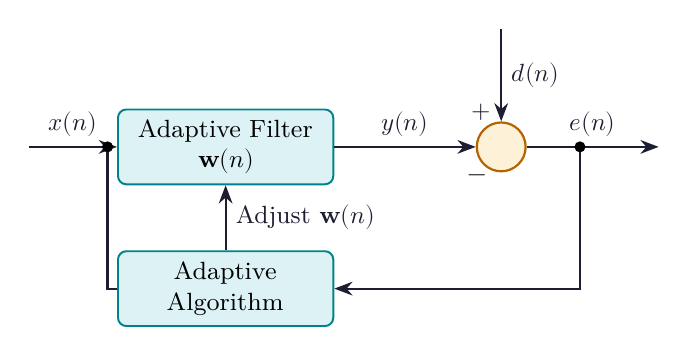
\begin{tikzpicture}[node distance=0.8cm and 1.2cm, every node/.style={font=\small}]
  \coordinate (input) at (-1.5, 0);
  \node[block, text width=2.5cm] (filter) at (1.0, 0) {Adaptive Filter\\$\mathbf{w}(n)$};
  \node[sumjunc] (sum) at (4.5, 0) {};
  \node[block, text width=2.5cm] (algo) at (1.0, -1.8) {Adaptive Algorithm};
  \coordinate (desired) at (4.5, 1.5);
  \coordinate (output) at (6.5, 0);
  
  \draw[arrow] (input) -- node[midway, above] {$x(n)$} (filter);
  \draw[line] (-0.5, 0) |- (algo.west);
  \fill (-0.5, 0) circle (2pt);
  
  \draw[arrow] (filter) -- node[midway, above] {$y(n)$} (sum);
  \draw[arrow] (desired) -- node[midway, right] {$d(n)$} node[pos=0.9, left] {$+$} (sum);
  \draw[arrow] (sum) -- node[midway, above] {$e(n)$} (output);
  \draw[arrow] (5.5, 0) |- (algo.east);
  \fill (5.5, 0) circle (2pt);
  
  \draw[arrow] (algo.north) -- node[midway, right] {Adjust $\mathbf{w}(n)$} (filter.south);
  \node at (4.2, -0.4) {$-$};
\end{tikzpicture}
\end{tcolorbox}

% ===============================================================================
\section{Applications and Motivation}
% ===============================================================================

The primary motivation for adaptive filtering is the inability of classical filter designs to operate in environments where the signal characteristics are either unknown or time-varying. Typical applications are categorized into four basic classes depending on the choice of input $x(n)$ and desired response $d(n)$:

\subsection{The Four Classes of Adaptive Filter Applications}

\begin{enumerate}[label=\textbf{\arabic*.}, leftmargin=*, itemsep=4pt]
  \item \textbf{System Identification:} The adaptive filter models the transfer function of an unknown system.
    \begin{itemize}[label=$\bullet$, leftmargin=*]
      \item \textit{Setup:} Input $x(n)$ is fed to both the unknown system and the adaptive filter. The system output is the desired response $d(n)$.
      \item \textit{Application:} Echo cancellation in long-distance telephony, channel characterization.
    \end{itemize}
  \item \textbf{Inverse Modeling (Equalization):} The filter is placed in cascade with an unknown channel to compensate for channel distortion.
    \begin{itemize}[label=$\bullet$, leftmargin=*]
      \item \textit{Setup:} A known training signal is sent. The distorted channel output is input $x(n)$, and the original training signal is the desired response $d(n)$.
      \item \textit{Application:} High-speed digital communication channel equalization.
    \end{itemize}
  \item \textbf{Noise Cancellation (Interference Cancellation):} The filter estimates and subtracts noise from a corrupted signal.
    \begin{itemize}[label=$\bullet$, leftmargin=*]
      \item \textit{Setup:} Input $x(n)$ is a reference noise source. The desired response $d(n)$ is the signal corrupted by noise.
      \item \textit{Application:} Active noise control, cancellation of maternal ECG in fetal monitoring.
    \end{itemize}
  \item \textbf{Linear Prediction:} The filter predicts future values of a random process.
    \begin{itemize}[label=$\bullet$, leftmargin=*]
      \item \textit{Setup:} Input $x(n)$ is a delayed version of the signal, and the desired response $d(n)$ is the current signal value.
      \item \textit{Application:} Linear Predictive Coding (LPC) in speech compression, ADPCM encoders.
    \end{itemize}
\end{enumerate}

\par\noindent
\begin{tabularx}{\linewidth}{|B{3.2cm}|Y|Y|Y|}
\hline
\rowcolor{hdrteal}
\textbf{Application Class} & \textbf{Input Signal $x(n)$} & \textbf{Desired Signal $d(n)$} & \textbf{Objective} \\
\hline
\textbf{System ID} & Reference excitation & Unknown system output & Find model $\mathbf{w}(n) \approx \text{system}$ \\
\hline
\rowcolor{rowalt}
\textbf{Inverse Model} & Distorted signal & Original source signal & Recover original source \\
\hline
\textbf{Noise Cancellation} & Noise reference source & Corrupted signal & Extract clean signal $e(n)$ \\
\hline
\rowcolor{rowalt}
\textbf{Prediction} & Delayed signal $s(n-\Delta)$ & Current signal $s(n)$ & Predict future signal values \\
\hline
\end{tabularx}

% ===============================================================================
\section{Review of Probability, Random Variables and Stationary Processes}
% ===============================================================================

Adaptive filter design relies heavily on statistical signal processing. This section reviews the prerequisite concepts of random signals.

\subsection{Random Variables and Probability Density Functions}
A random variable $X$ is a mapping from sample space to real numbers. It is described by its Probability Density Function (PDF) $f_X(x)$.
\begin{itemize}[leftmargin=*, itemsep=2pt]
  \item \textbf{Expectation (Mean):} The statistical average of $X$:
  \begin{equation}
    \mu_X = \mathbb{E}[X] = \int_{-\infty}^{\infty} x f_X(x) \, dx
  \end{equation}
  \item \textbf{Variance:} The measure of signal spread/power:
  \begin{equation}
    \sigma_X^2 = \mathbb{E}[(X - \mu_X)^2] = \mathbb{E}[X^2] - \mu_X^2
  \end{equation}
\end{itemize}

\subsection{Stationary and Ergodicity}
A random process $X(n)$ is a collection of random variables indexed by time.
\begin{itemize}[leftmargin=*, itemsep=3pt]
  \item \textbf{Strict-Sense Stationarity (SSS):} A process is SSS if its joint probability distributions are invariant to any shift in the time origin.
  \item \textbf{Wide-Sense Stationarity (WSS):} A process is WSS if:
    \begin{enumerate}[label=\textbf{\alph*.}, leftmargin=*, itemsep=1pt]
      \item Its mean is constant over time: $\mathbb{E}[X(n)] = \mu$
      \item Its autocorrelation depends only on the time difference (lag) $k$:
      \begin{equation}
        R_x(k) = \mathbb{E}[X(n) X^*(n-k)]
      \end{equation}
    \end{enumerate}
  \item \textbf{Ergodicity:} A WSS process is ergodic if its time averages equal its ensemble averages. This allows computing statistical metrics from a single, long time realization.
\end{itemize}

% ===============================================================================
\section{Correlation Structures and Correlation Matrices}
% ===============================================================================

Let $\mathbf{x}(n) = [x(n), x(n-1), \dots, x(n-M+1)]^T$ be an $M \times 1$ tap-input vector of a WSS process. The statistical relationship among its elements is captured by the autocorrelation matrix $\mathbf{R}$.

\subsection{The Autocorrelation Matrix}
The autocorrelation matrix $\mathbf{R}$ is defined as:
\begin{equation}
  \mathbf{R} = \mathbb{E}[\mathbf{x}(n) \mathbf{x}^H(n)]
\end{equation}
where $^H$ denotes the Hermitian transpose (conjugate transpose). In expanded form:
\begin{equation}
  \mathbf{R} = \begin{bmatrix}
    R_x(0) & R_x(1) & \dots & R_x(M-1) \\
    R_x(-1) & R_x(0) & \dots & R_x(M-2) \\
    \vdots & \vdots & \ddots & \vdots \\
    R_x(-M+1) & R_x(-M+2) & \dots & R_x(0)
  \end{bmatrix}
\end{equation}
Since the process is WSS, $R_x(-k) = R_x^*(k)$.

\subsection{Properties of the Correlation Matrix}
The matrix $\mathbf{R}$ possesses several fundamental properties that dictate the behavior of adaptive filters:
\begin{enumerate}[label=\textbf{\arabic*.}, leftmargin=*, itemsep=4pt]
  \item \textbf{Hermitian Symmetry:} $\mathbf{R}$ is Hermitian, i.e., $\mathbf{R}^H = \mathbf{R}$.
  \item \textbf{Toeplitz Structure:} All elements along any main diagonal are identical. This symmetry reduces computational cost for matrix inversion algorithms.
  \item \textbf{Positive Semi-Definiteness:} For any non-zero complex vector $\mathbf{a}$:
  \begin{equation}
    \mathbf{a}^H \mathbf{R} \mathbf{a} = \mathbf{a}^H \mathbb{E}[\mathbf{x}(n)\mathbf{x}^H(n)]\mathbf{a} = \mathbb{E}[|\mathbf{a}^H\mathbf{x}(n)|^2] \ge 0
  \end{equation}
  If no component of the input signal is perfectly predictable, $\mathbf{R}$ is positive definite ($\mathbf{a}^H \mathbf{R} \mathbf{a} > 0$), meaning all its eigenvalues are strictly positive ($\lambda_i > 0$), ensuring $\mathbf{R}$ is invertible.
  \item \textbf{Eigenvalue Bounds:} The eigenvalues of $\mathbf{R}$ are bounded by the minimum and maximum values of the Power Spectral Density (PSD) of the input process:
  \begin{equation}
    S_{\text{min}} \le \lambda_i \le S_{\text{max}}
  \end{equation}
\end{enumerate}

\begin{tcolorbox}[examplebox, title={Example: Correlation Matrix of a Sinusoid with Noise}]
Consider an input signal $x(n) = A \cos(\omega_0 n + \theta) + v(n)$, where $\theta$ is uniformly distributed in $[-\pi, \pi]$ and $v(n)$ is zero-mean white noise with variance $\sigma_v^2$ uncorrelated with the sinusoid. Compute the autocorrelation matrix for $M = 2$.

\textbf{Solution:}
The autocorrelation function of the sinusoid is $R_s(k) = \frac{A^2}{2}\cos(\omega_0 k)$.
The autocorrelation function of the white noise is $R_v(k) = \sigma_v^2 \delta(k)$.
Since they are uncorrelated, the total autocorrelation is:
\[
  R_x(k) = R_s(k) + R_v(k) = \frac{A^2}{2}\cos(\omega_0 k) + \sigma_v^2 \delta(k)
\]
For $k=0$ and $k=1$:
\[
  R_x(0) = \frac{A^2}{2} + \sigma_v^2
\]
\[
  R_x(1) = \frac{A^2}{2}\cos(\omega_0)
\]
Thus, the $2 \times 2$ correlation matrix is:
\[
  \mathbf{R} = \begin{bmatrix}
    \frac{A^2}{2} + \sigma_v^2 & \frac{A^2}{2}\cos(\omega_0) \\
    \frac{A^2}{2}\cos(\omega_0) & \frac{A^2}{2} + \sigma_v^2
  \end{bmatrix}
\]
\end{tcolorbox}

% ===============================================================================
% MANDATORY QUICK REVISION PAGE
% ===============================================================================
\newpage
\begin{center}
  {\large\bfseries\color{myred} Quick Revision --- Module I}\\[3pt]
  {\small\color{mydark} Adaptive Filtering Concepts \& Random Processes $|$ PE-EC702A}
\end{center}
\noindent{\color{myred}\rule{\linewidth}{1.2pt}}
\vspace{4pt}

\begin{tcolorbox}[formulabox, title={\textbf{Key Formulas at a Glance}}]
\renewcommand{\arraystretch}{1.3}
\begin{tabularx}{\linewidth}{B{4.5cm} X}
Filter Output (FIR) & $y(n) = \mathbf{w}^T(n)\mathbf{x}(n) = \sum_{k=0}^{M-1} w_k(n) x(n-k)$ \\[6pt]
Error Signal & $e(n) = d(n) - y(n)$ \\[6pt]
Autocorrelation Function & $R_x(k) = \mathbb{E}[x(n) x^*(n-k)]$ \\[6pt]
Correlation Matrix & $\mathbf{R} = \mathbb{E}[\mathbf{x}(n) \mathbf{x}^H(n)]$ \\[6pt]
Cross-Correlation Vector & $\mathbf{p} = \mathbb{E}[\mathbf{x}(n) d^*(n)]$
\end{tabularx}
\end{tcolorbox}

\begin{tcolorbox}[defbox, title={\textbf{One-Line Definitions}}]
\begin{itemize}[leftmargin=*, itemsep=2.5pt, topsep=0pt]
  \item \textbf{Adaptive Filter:} A digital filter that dynamically self-adjusts its coefficients to minimize a cost function.
  \item \textbf{Desired Response:} The target reference signal that the adaptive filter output attempts to replicate.
  \item \textbf{Wide-Sense Stationarity:} A process with constant mean and an autocorrelation depending only on lag.
  \item \textbf{Ergodicity:} A property where time-average statistics are identical to ensemble-average statistics.
  \item \textbf{Toeplitz Matrix:} A matrix where elements on each diagonal are constant, characteristic of WSS correlation matrices.
  \item \textbf{Hermitian Matrix:} A complex matrix equal to its own conjugate transpose, $\mathbf{R}^H = \mathbf{R}$.
\end{itemize}
\end{tcolorbox}

\begin{tcolorbox}[exambox, title={\textbf{Frequently Asked / Viva Questions}}]
\begin{enumerate}[topsep=0pt, label=\textbf{Q\arabic*.}, itemsep=5pt]
  \item \Q{What is the primary difference between a fixed filter and an adaptive filter?}
    Fixed filters have static coefficients designed based on prior knowledge of signal spectra, whereas adaptive filters continuously update their coefficients in real-time based on statistical changes in the input signals.
  \item \Q{Explain the role of the desired response $d(n)$ in an adaptive system.}
    The desired response acts as a target reference signal. The difference between $d(n)$ and the filter output $y(n)$ produces the error $e(n)$, which guides the optimization algorithm.
  \item \Q{Identify the four main application classes of adaptive filters.}
    System Identification, Inverse Modeling (Equalization), Noise Cancellation, and Linear Prediction.
  \item \Q{Why does the autocorrelation matrix $\mathbf{R}$ of a WSS process possess Toeplitz structure?}
    Because for a WSS process, the autocorrelation between $x(i)$ and $x(j)$ depends strictly on the lag $|i - j|$, causing elements along any diagonal to be identical.
  \item \Q{State the significance of the positive definite property of a correlation matrix.}
    Positive definiteness implies that all eigenvalues of $\mathbf{R}$ are strictly positive ($\lambda_i > 0$), which guarantees that the matrix is non-singular and hence invertible.
  \item \Q{What is ensemble average vs time average?}
    Ensemble average is the average across all possible realizations of a random variable at a specific time, while time average is computed along a single realization over infinite time.
  \item \Q{Define a Hermitian matrix in the context of adaptive filtering.}
    A matrix $\mathbf{R}$ is Hermitian if $\mathbf{R}^H = \mathbf{R}$ (where $^H$ denotes the conjugate transpose). The autocorrelation matrix of any complex random process is always Hermitian.
  \item \Q{What is the physical interpretation of $R_x(0)$?}
    $R_x(0) = \mathbb{E}[|x(n)|^2]$, which represents the average total power of the input signal $x(n)$.
  \item \Q{What happens to the eigenvalues of $\mathbf{R}$ if the input is white noise?}
    All eigenvalues of the correlation matrix of white noise are identical and equal to the noise variance ($\lambda_i = \sigma^2$).
  \item \Q{What is the cross-correlation vector $\mathbf{p}$?}
    It is the statistical correlation vector between the input signal vector $\mathbf{x}(n)$ and the desired response $d(n)$, defined as $\mathbf{p} = \mathbb{E}[\mathbf{x}(n) d^*(n)]$.
\end{enumerate}
\end{tcolorbox}

\begin{tcolorbox}[tikzbox, title={Comparison of Adaptive Filter Application Classes}]
\renewcommand{\arraystretch}{1.4}
\par\noindent
\begin{tabularx}{\linewidth}{|B{2.8cm}|Y|Y|Y|}
\hline
\rowcolor{hdrgray}
\textbf{Parameter} & \textbf{System ID} & \textbf{Noise Cancellation} & \textbf{Equalization} \\
\hline
\textbf{Filter Input $x(n)$} & Excitation signal & Reference noise source & Distorted channel output \\
\hline
\textbf{Desired Input $d(n)$} & Output of unknown system & Corrupted signal & Known training signal \\
\hline
\textbf{Desired Output} & Model of system parameters & Cleaned signal $e(n)$ & Reconstructed original data \\
\hline
\textbf{Key Application} & Echo cancellation in telephony & Active noise control, EEG & Wireless communications \\
\hline
\end{tabularx}
\end{tcolorbox}

\end{document}
